% QCE26 NIER short paper.
% Named build:     latexmk -pdf -interaction=nonstopmode -halt-on-error main.tex
% Anonymous build: latexmk -pdf -interaction=nonstopmode -halt-on-error main_anon.tex
\documentclass[10pt,conference]{IEEEtran}
\IEEEoverridecommandlockouts

\usepackage[T1]{fontenc}
\usepackage[utf8]{inputenc}
\usepackage{microtype}
\usepackage{amsmath,amssymb}
\usepackage{graphicx}
\graphicspath{{gfx/}{figures/}}
\usepackage{booktabs}
\usepackage{balance}
\usepackage{cite}
\usepackage{xcolor}
\definecolor{paperblue}{HTML}{0057FF}
\definecolor{citegreen}{HTML}{39FF14}
\usepackage[hypertexnames=false]{hyperref}
\usepackage{orcidlink}
\hypersetup{%
  colorlinks=true,
  linkcolor=paperblue,
  citecolor=citegreen,
  urlcolor=paperblue,
  pdfborder={0 0 0},
  pdftitle={From Quantum Shots to Training Data: Reorganizing Measurement Records for Improved Finite-Shot Quantum Learning},
  pdfsubject={QCE26 NIER short paper on validation based measurement aggregation for quantum reservoir computing},
  pdfkeywords={quantum reservoir computing, finite shot learning, measurement aggregation, time series forecasting}
}
\urlstyle{same}

\newcommand{\nrmse}{\mathrm{NRMSE}}
\newcommand{\Grouped}{Grouped}
% Manuscript-facing outcomes from the evidence-preserving merge in
% results/qai_robust_protocol_santa_fe_manuscript/.
\newcommand{\QAIFeatureDimension}{11}
\newcommand{\QAIFeatureEffectiveRank}{5.15}

\newcommand{\QAIMackeyEVGrouped}{0.0445}
\newcommand{\QAIMackeyEVGroupedLow}{0.0372}
\newcommand{\QAIMackeyEVGroupedHigh}{0.0519}
\newcommand{\QAISantaFeEVGrouped}{0.0848}
\newcommand{\QAISantaFeEVGroupedLow}{0.0174}
\newcommand{\QAISantaFeEVGroupedHigh}{0.1522}
\newcommand{\QAIRosslerEVGrouped}{0.0349}
\newcommand{\QAIRosslerEVGroupedLow}{0.0139}
\newcommand{\QAIRosslerEVGroupedHigh}{0.0559}
\newcommand{\QAISunspotsEVGrouped}{0.0360}
\newcommand{\QAISunspotsEVGroupedLow}{0.0103}
\newcommand{\QAISunspotsEVGroupedHigh}{0.0616}

% Protocol-matched Santa Fe hardware extension. The intervals are descriptive
% paired intervals over twenty disjoint shot blocks within one acquisition.
\newcommand{\QAIHardwareFezSantaEV}{0.750}
\newcommand{\QAIHardwareFezSantaGrouped}{0.711}
\newcommand{\QAIHardwareFezSantaGain}{0.038}
\newcommand{\QAIHardwareFezSantaGainLow}{0.027}
\newcommand{\QAIHardwareFezSantaGainHigh}{0.050}
\newcommand{\QAIHardwareMarrakeshSantaEV}{0.744}
\newcommand{\QAIHardwareMarrakeshSantaGrouped}{0.713}
\newcommand{\QAIHardwareMarrakeshSantaGain}{0.031}
\newcommand{\QAIHardwareMarrakeshSantaGainLow}{0.023}
\newcommand{\QAIHardwareMarrakeshSantaGainHigh}{0.039}
\newcommand{\QAIHardwareSantaWins}{19/20}
\newcommand{\QAIHardwareFezSeconds}{55}
\newcommand{\QAIHardwareMarrakeshSeconds}{56}
\newcommand{\QAIHardwareTotalSeconds}{111}

% Balanced-setting means in the order Classical, Ideal QRC, EV, Grouped, Raw, Regularized EV from
% results/qai_robust_protocol_santa_fe_manuscript/cluster_summary.csv.
\newcommand{\QAIBalancedTableRows}{%
Mackey--Glass & 0.098 & 0.190 & 0.484 & 0.439 & 0.586 & \textbf{0.430} \\
Santa Fe laser & 0.762 & 0.493 & 0.764 & 0.680 & 0.697 & \textbf{0.677} \\
R\"ossler & 0.096 & 0.054 & 0.414 & 0.379 & 0.580 & \textbf{0.367} \\
Sunspots & 0.387 & 0.474 & 0.553 & 0.517 & 0.558 & \textbf{0.515} \\
}

\setlength{\textfloatsep}{7pt plus 1pt minus 2pt}
\setlength{\abovecaptionskip}{4pt}
\setlength{\dbltextfloatsep}{7pt plus 1pt minus 2pt}
\setlength{\floatsep}{6pt plus 1pt minus 1pt}

\begin{document}

\title{From Quantum Shots to Training Data:\\
Reorganizing Measurement Records for Improved Finite-Shot Quantum Learning}

\ifdefined\ANON
  \hypersetup{pdfauthor={}}
  \author{\IEEEauthorblockN{Anonymous Authors}}
\else
  \hypersetup{pdfauthor={Markus Baumann; Maximilian Zorn; Thomas Gabor; Claudia Linnhoff-Popien; Jonas Stein}}
  \author{%
  \IEEEauthorblockN{%
  Markus Baumann\IEEEauthorrefmark{1}\orcidlink{0009-0007-3575-1006}\thanks{Corresponding author: \href{mailto:markus.baumann@campus.lmu.de}{markus.baumann@campus.lmu.de}.},
  Maximilian Zorn\IEEEauthorrefmark{1}\orcidlink{0009-0006-2750-7495},
  Thomas Gabor\IEEEauthorrefmark{2}\orcidlink{0000-0003-2048-8667},
  Claudia Linnhoff-Popien\IEEEauthorrefmark{1}\orcidlink{0000-0001-6284-9286},
  and Jonas Stein\IEEEauthorrefmark{1}\orcidlink{0000-0001-5727-9151}}
  \IEEEauthorblockA{\IEEEauthorrefmark{1}\textit{QAR-Lab, Department of Computer Science, LMU Munich, Munich, Germany}\\
  \IEEEauthorrefmark{2}\textit{Department of Computer Science, University of Exeter, Exeter, United Kingdom}}
  }
\fi

\maketitle
\bstctlcite{BSTcontrol}

\begin{abstract}
Between keeping every shot as a noisy training example and averaging all shots
into one clean feature lies an entire spectrum of data organizations that
quantum machine learning usually leaves implicit. We make that choice explicit.
Shot grouping partitions a fixed measurement record into disjoint groups and
averages within each group, tuning smoothly between the two conventions with a
single validated parameter and no additional quantum executions. We evaluate
the method on chaotic synthetic benchmarks and on real-world data under strict
execution budgets. An intermediate grouping consistently outperforms the
standard expectation-value pipeline. Matched controls show that the gain acts
as correctly scaled regularization of the classical readout. Unmitigated runs
on two superconducting processors confirm the trend on every task. Shot
grouping therefore offers a practical way to improve finite-shot quantum
learning at no added quantum cost.
\end{abstract}

\begin{IEEEkeywords}
quantum reservoir computing, finite shot learning, measurement aggregation,
time series forecasting
\end{IEEEkeywords}

\section{Introduction}
\label{sec:introduction}

Every quantum learning experiment ends the same way: a circuit runs many
times, and each run returns one measured bitstring. Before anything can be
learned, this pile of shots must become training data. The step looks like
bookkeeping, and it is usually treated that way. Almost every pipeline averages
all shots of a time step into a single expectation-value estimate and moves on.
This paper argues that the step is not bookkeeping. It is a statistical decision
with measurable consequences, and treating it as a validated hyperparameter
improves finite-shot quantum learning at no additional quantum cost.

\begin{figure}[!t]
  \centering
  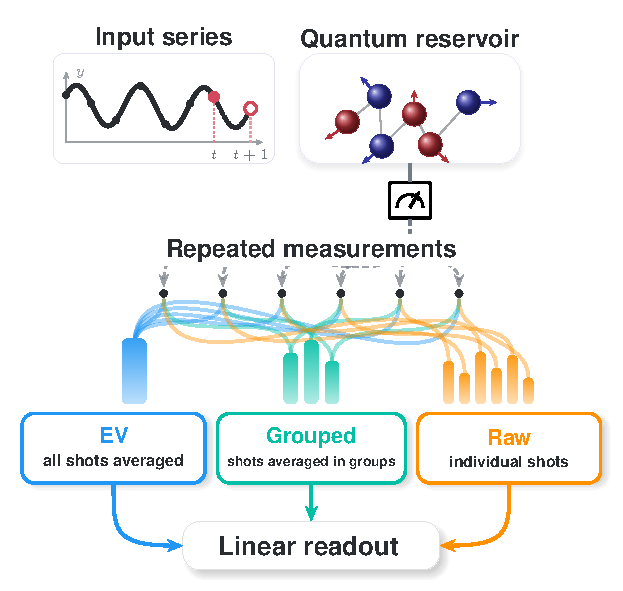
\includegraphics[width=\columnwidth]{fig1_shot_organization.pdf}
  \caption{Three ways to turn one shot record into training data. A fixed quantum
  reservoir is measured many times per step, and only the classical step changes:
  EV averages all shots, Raw keeps each shot, and Grouped averages disjoint groups.
  All feed the same linear readout.}
  \label{fig:organization}
\end{figure}

The averaging convention is well motivated, because expectation values are the
quantities predicted by theory and estimated in experiments. A learning
pipeline, however, does not consume observables. It consumes training examples,
and it cares about two things only: how many there are and how noisy each one is.
The moment a measurement record becomes training data, a physics convention
quietly turns into a statistical choice: spend all measurements on making one
example clean, or make several examples that are merely clean enough. No single
choice can suit every task, budget, and noise level.

Averaging everything is one end of a dial. It buys the cleanest possible feature
vector but pays with scarcity: thousands of circuit executions collapse into a
handful of training examples, and too few examples relative to the number of
features destabilizes regression~\cite{hsu2012random}. The opposite end, keeping
every shot as its own example, buys abundance but pays with noise, and noisy
features systematically shrink fitted coefficients~\cite{fuller1987measurement}.
Between these extremes lies an entire range of aggregations that quantum machine
learning usually leaves implicit.

\emph{Adaptive shot aggregation} makes this choice explicit. The $N$ shots of
each time step are partitioned into disjoint groups of size $k$ and averaged
within each group, so that a single parameter slides smoothly from raw shots
($k=1$) to full expectation-value averaging ($k=N$). The group size is a
validation-selected hyperparameter of the classical readout, chosen by
time-respecting validation jointly with the readout regularization. The
procedure operates purely on the classical record: it requires no new circuits,
no extra shots, and it can be applied retroactively to any archived record in
which individual outcomes were retained.

Quantum reservoir computing (QRC) is a clean place to study this
dial~\cite{fujii2017harnessing,nakajima2019boosting,mujal2021opportunities}. A
fixed quantum circuit transforms an input sequence into measured features, and
only a classical readout is trained. The circuit, the targets, and the
measurement record can therefore be held completely fixed while the aggregation
alone changes. Whatever happens to the forecast is attributable to the
aggregation, because nothing else moved. We compare three representations of
one record (Fig.~\ref{fig:organization}): the expectation-value representation
(EV), individual shots (Raw), and the grouped representation in between.

We find that the aggregation scale materially affects test error under fixed
execution budgets: at the balanced allocation, an intermediate scale lowers
mean test error relative to full averaging on all four evaluated forecasting
tasks, with paired confidence intervals above zero in every case. The best scale
depends on the record, so no single convention is appropriate. Matched controls
trace the gain to covariance regularization of the classical readout, supplied
automatically by the record's own shot fluctuations, and the effect transfers
to unmitigated experiments on real hardware. Our claims concern how to organize
a given measurement record, not quantum advantage.

In summary, this paper makes the following contributions:

\begin{itemize}
  \setlength{\itemsep}{1pt}
  \setlength{\parskip}{0pt}
  \setlength{\parsep}{0pt}
  \setlength{\topsep}{2pt}
  \item \textbf{A tunable aggregation procedure.} We make $k$ a
  validation-selected classical-readout hyperparameter spanning Raw to EV,
  chosen jointly with ridge strength and applicable retroactively at no added
  quantum cost (Sec.~\ref{sec:method}).

  \item \textbf{Evidence that the choice matters.} Under a fixed budget of
  10,000 executions, intermediate aggregation lowers mean error on all four
  tasks; a three-allocation sweep shows that gains are largest with many shots
  at few time steps
  (Secs.~\ref{sec:evaluation}-A and \ref{sec:evaluation}-B).

  \item \textbf{A mechanism.} An exact linear-readout identity equates grouped
  training with EV training plus a shot-covariance penalty; the matched
  Regularized EV control confirms this mechanism
  (Secs.~\ref{sec:method}-C and \ref{sec:evaluation}-C).

  \item \textbf{Transfer to hardware.} Unmitigated experiments with a separate
  ten-qubit reservoir on two processors show positive mean improvements on
  every task (Sec.~\ref{sec:evaluation}-D).
\end{itemize}

\section{Related Work}
\label{sec:related}

Finite sampling can be addressed at three points in a quantum learning
pipeline. It can be addressed before execution, by deciding how to spend a
measurement budget. It can be addressed after averaging, by correcting the
statistics of expectation values. Or it can be addressed at the record
itself, by changing how repeated measurements become training data. Our
method lives at this third point, which is the least studied of the three.

The idea of averaging subsets of measurements is not new, and we do not claim
it. Cemin \emph{et al.} average subsets of measurements to enlarge a training
set for reduced quantum channel learning~\cite{cemin2024channels}, and it is
a classical result that training with noisy inputs behaves like an additional
penalty on large fitted weights~\cite{bishop1995training}. What has been
missing is the treatment of the aggregation scale as a tunable quantity. This
study evaluates the complete range from Raw to EV on one fixed QRC record,
calibrates the scale jointly with the readout regularization, gives an exact
account of the penalty this creates, and tests the result under three
allocations of a fixed execution budget on four matched forecasting tasks.
The contribution is the calibration and evaluation of the aggregation scale,
not the original introduction of subset averaging.

The other two points of the pipeline are well developed and complementary to
ours. Before execution, resource-aware optimization decides how many
measurements each part of a computation deserves~\cite{moussa2023resource}.
After averaging, Ahmed \emph{et al.} derive noise-aware training rules for
expectation values~\cite{ahmed2025optimal}, and Kreplin and Roth reduce
sampling noise through variance regularization~\cite{kreplin2024reduction}.
Fundamental limits of learning from finitely sampled physical systems have
also been mapped out~\cite{hu2023tackling}. None of these methods competes
with ours. Allocation ends where our method begins, and the averaged
quantities that noise-aware corrections operate on can themselves be produced
by grouped aggregation. Our method needs nothing beyond a single archived
measurement record.

Within QRC, a rich line of work studies how noise, dissipation, measurement,
finite Hilbert space, and input transformations shape temporal
features~\cite{kubota2022noise,palacios2024role,kubota2023temporal,martinezpena2023finite,mujal2023timeseries,suzuki2022natural,sannia2024dissipation,govia2022nonlinear,martinezpena2023capacity,kalfus2022hilbert,fry2023noiseinduced,govia2021singleoscillator}.
All of these studies analyze or modify the quantum representation. We do the
opposite. The representation is held completely fixed, and only the
organization of its repeated measurements changes. Because every reservoir in
those studies still produces a measurement record, adaptive shot aggregation
applies on top of any of them.

\section{Method}
\label{sec:method}

\subsection{Simulation reservoir}

The reservoir has six qubits and two shallow data reuploading layers
~\cite{perezsalinas2020data}. Each layer encodes the scalar input on every
qubit with heterogeneous $R_y$ and $R_z$ rotations, applies neighboring
$R_{zz}$ couplings, and mixes locally with frozen non-Clifford angles. The
circuit parameters are fixed before forecasting, and additional frozen
realizations quantify sensitivity. One computational basis measurement yields
six local $Z_i$ signs and five neighboring products $Z_iZ_{i+1}$ at no
additional quantum cost.

Ideal statevector simulation is performed before forecasting. All 11 features
change with the input and exceed the specified nonlinearity threshold. They
all contribute distinct numerical information. Because several respond in
similar ways, their effective number is 5.15. A leak of 0.2
and ten causal lags provide temporal context. Ridge regression produces the
next step forecast, and performance is measured by test NRMSE. These checks
show that the reservoir supplies a varied, nonlinear feature set. They do not evaluate
quantum advantage.

\subsection{Adaptive shot aggregation}

Let $x_t^{(n)}$ denote the processed features from shot index $n$ at time
$t$. For a divisor $k$ of $N$, the $N$ shots are partitioned into
$G=N/k$ disjoint groups, producing
\begin{equation}
  x_t^{(g)}=\frac{1}{k}\sum_{n\in g}x_t^{(n)},
  \qquad g=1,\ldots,G .
  \label{eq:grouping}
\end{equation}
Each grouped sample shares the same target. At evaluation, the $G$
predictions for one step are averaged. This equals prediction from their mean
features, so any difference between EV and Grouped is created during
training rather than evaluation.

Measurement indices do not identify physical trajectories. A random
permutation is therefore drawn at every time step before groups are formed, and
the analysis is repeated across random grouping assignments. A fixed assignment across time
is included as a sensitivity analysis.

\subsection{Fixed execution budget and training}

The quantum cost is $TN$ circuit executions. Three specified settings use
exactly $10{,}000$ executions. They allocate $(T,N)=(250,40)$, $(500,20)$, and
$(1000,10)$ to the number of time steps and shots. All divisors of $N$ are
considered, including Raw at $k=1$ and EV at $k=N$. Three expanding
train-and-check splits preserve time order: each candidate pair $(k,\lambda)$
is fitted on an earlier block and scored on the following block. The best pair
is then fixed, the readout is refitted to all data preceding the test block,
and the final 20\% is evaluated once. Normalization and feature scaling use
training data only.

\subsection{Why grouping regularizes the readout}
\label{sec:mechanism}

Full averaging gives the readout one clean view of each time step. Individual
shots give it many views, but every view is noisy. Intermediate groups provide
several partially denoised versions of the same target. Differences among
those versions reveal which feature changes are stable across shots and which
are measurement noise. Training on all grouped versions discourages the
readout from relying on the unstable changes.

For a linear readout with squared loss, this intuition can be written as an
exact identity. Let $\bar{x}_t$ be the mean of the $G$ grouped
views and let
$C_{k,t}=G^{-1}\sum_g(x_t^{(g)}-\bar{x}_t)(x_t^{(g)}-\bar{x}_t)^\top$.
This quantity summarizes how the measured features fluctuate together around
their mean. For intercept $b$ and weights $w$,
\begin{equation}
 \frac{1}{G}\sum_g\!\left(y_t-b-w^\top x_t^{(g)}\right)^2
 =\left(y_t-b-w^\top\bar{x}_t\right)^2+w^\top C_{k,t}w .
 \label{eq:covariance}
\end{equation}
The first term on the right is the EV loss. The second adds a larger cost when
the readout relies on combinations of features that vary strongly across the
grouped views. Grouped training is therefore exactly EV training plus a
penalty determined by the observed shot fluctuations. This identity requires
neither Gaussian noise nor independence across time.

Cov-EV applies the same fluctuation-based penalty directly to EV and chooses
its strength separately using the same earlier data as Grouped. If both methods
perform similarly, the benefit of grouping is explained by this regularization
rather than by additional physical information. We also compute both forms at
fixed $k$ and confirm identical predictions as an implementation check.
The leaky integrator and overlapping lags make adjacent feature sets
dependent, so uncertainty is computed over trajectories or measured windows,
not over the many grouped views. The full derivation and statistical details are
provided in the supplement.

\section{Experimental Setup}
\label{sec:setup}

We run two studies. The first is a controlled simulation on four forecasting
tasks. The second repeats the core comparison on real quantum hardware. In both,
every aggregation choice reads the very same measurement record, so any
difference in accuracy comes only from how the shots are organized and not from
running the circuit differently.

\subsection{Simulation reservoir and evaluation protocol}

The simulated reservoir is a fixed six-qubit circuit with two shallow data
reuploading layers~\cite{perezsalinas2020data}. Each layer applies
input-dependent $R_y$ and $R_z$ rotations with fixed per-qubit offsets,
nearest-neighbor $R_{zz}$ couplings, and fixed non-Clifford mixing rotations.
For each circuit setting, all angles are sampled once and then held fixed;
three frozen settings are used to assess sensitivity to this draw. Each
computational-basis shot yields 11 features: six local observables $Z_i$ and
five nearest-neighbor products $Z_iZ_{i+1}$. A leaky integrator with leak rate
$0.2$ and a ten-step lag window provide temporal memory, and a ridge-regression
readout predicts the next value.

We evaluate one-step-ahead forecasting on four time series: the synthetic
Mackey--Glass~\cite{mackey1977oscillation} and
R\"ossler~\cite{rossler1976equation} systems, and the measured Santa Fe laser
intensity~\cite{gershenfeld1993future} and monthly sunspot
number~\cite{sidc2026sunspots}. All tasks use the same reservoir architecture,
feature construction, temporal processing, scaling, validation procedure, and
execution budgets. The same selection rule is applied separately to each task;
no task-specific changes are made to the reservoir or preprocessing pipeline.

All four finite-shot methods use the same measurement record. Two additional
controls use different feature sources: an ideal reservoir without
finite-shot sampling noise and a classical baseline that applies the same
temporal processing and readout directly to the input series. These controls
distinguish the effect of aggregation from the effects of finite sampling and
of the reservoir transformation itself.

The trajectory or time window is the unit of uncertainty estimation.
Mackey--Glass uses twenty independently generated trajectories, each with a
held-out test block. R\"ossler uses five trajectories, and each real-world task
uses five windows with disjoint test blocks.
Within each unit,
we repeat the analysis over three circuit settings, three measurement draws,
and three random groupings where applicable. These repeats are averaged within
the unit before paired confidence intervals are formed across the independent
units for that task.
Grouped views, neighboring time steps, and repeated evaluations of the same
sequence are not treated as independent observations, because they share
measurements or are coupled by the leaky integrator and overlapping lags.

Model selection uses no test data. After a short washout, the final 20\% of each
trajectory or window is reserved as an untouched test block. The preceding
data are used in three expanding-window validation splits, each trained on the
available past and evaluated on the immediately following block. The group
size $k$ and ridge strength $\lambda$ are selected from these validation
results. The readout is then refitted on all data preceding the test block and
evaluated once on the reserved block. For representations with multiple views
at one time step, the corresponding predictions are averaged to produce one
forecast, so all methods are scored on the same targets.

The primary budget uses $T=500$ time steps and $N=20$ shots per step, giving
10,000 circuit executions. We also test $(T,N)=(250,40)$ and $(1000,10)$,
which spend the same budget with different balances between observed time
steps and shots per step. All reservoir parameters, data-generation settings,
window origins, and selection rules are fixed and stored before any test block
is evaluated.

\subsection{Hardware setup}
The hardware study uses a different reservoir: a fixed ten-qubit circuit with
one input qubit, nine memory qubits, a ring of entangling gates, and ten local
outputs mapped on \emph{ibm\_fez} and \emph{ibm\_marrakesh}. It tests transfer of
the aggregation procedure; it is not a hardware implementation of the six-qubit
simulator or a comparison of qubit counts. Every method receives the same
circuit outputs. For each task and processor, one acquisition of $400$ shots at $500$ time steps is
split into twenty ordered, disjoint records of $20$ shots. The intervals measure
variation within that acquisition, not across devices or calibration periods.

\begin{figure}[!t]
  \centering
  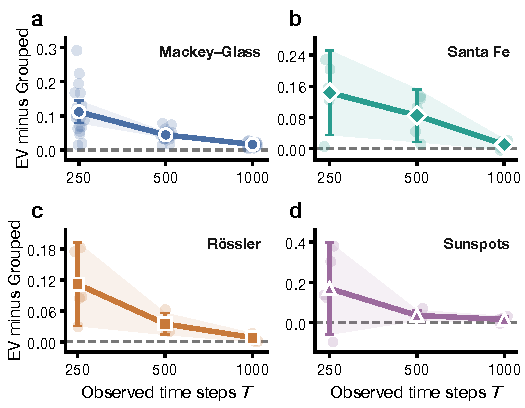
\includegraphics[width=\columnwidth]{fig3_regime_map.pdf}
  \caption{Fixed-budget allocation. Panels show EV-minus-Grouped NRMSE, so
  positive values favor Grouped. Moving right spends the budget on more steps
  and fewer shots; gains are largest with many shots and few steps. Markers and
  bars are means and 95\% intervals.}
  \label{fig:regimes}
\end{figure}

\section{Evaluation}
\label{sec:evaluation}

We report accuracy as test NRMSE, a normalized error for which lower is better
and where one means predicting the mean. Three ways of turning the shot record
into features are compared throughout. EV averages all shots of a step into one
clean feature vector. Raw keeps every shot as its own noisy example. Grouped is
our method and sits between them. A fourth entry, Cov-EV, is a control that adds
an independently tuned covariance penalty to plain averaging. We summarize the
benefit of Grouped as the paired difference EV minus Grouped, so a positive
value means Grouped is more accurate. Each difference comes with a $95\%$
confidence interval. An interval above zero provides evidence of a positive
mean improvement; an interval containing zero is inconclusive. The balanced
setting spends the fixed budget on $500$ time steps with $20$ shots each.

\subsection{Balanced setting}

At the balanced budget, Grouped lowers mean NRMSE relative to EV on all four
tasks (Table~\ref{tab:balanced}, Fig.~\ref{fig:operating}). The improvement is
$0.0138$ on Mackey--Glass ($95\%$ CI $[-0.0023, 0.0300]$), $0.0848$ on Santa Fe
laser ($[0.0174, 0.1522]$), $0.0349$ on R\"ossler ($[0.0139, 0.0559]$), and
$0.0360$ on sunspots ($[0.0103, 0.0616]$). The interval stays above zero on the
two real-world datasets, Santa Fe laser and sunspots, and on R\"ossler. Only
Mackey--Glass is inconclusive.

\begin{table}[t]
\caption{Mean test NRMSE at the balanced setting. Repeated measurement trials
are averaged within each of five separate trajectories or windows. Lower
values are better.}
\label{tab:balanced}
\centering
\scriptsize
\setlength{\tabcolsep}{1.7pt}
\begin{tabular}{lrrrrrr}
\toprule
Task & Class. & Ideal & EV & Grouped & Raw & Cov-EV \\
\midrule
\QAIBalancedTableRows
\bottomrule
\end{tabular}
\end{table}

Santa Fe laser shows the largest effect. Grouped reduces the error from $0.764$
to $0.680$, and all five disjoint test windows favor Grouped. When $k$ and the
ridge strength are tuned together, the search lands on $k=10$ most often and
on an intermediate scale, neither Raw nor EV, in $94\%$ of repeated trials.
Cov-EV reaches $0.677$, almost the same as Grouped, which already suggests that
the gain is a regularization effect rather than new physical information. The
gain also depends on how the budget is spent. On Santa Fe it shrinks from
$0.143$ with $40$ shots per step to $0.010$ with $10$ shots per step because
grouping has more shots to reorganize when shots are plentiful.

We also compare an ideal noise-free reservoir with a classical baseline that
uses identical preprocessing. The quantum reservoir is worse on Mackey--Glass
and sunspots, better on Santa Fe, and inconclusive on R\"ossler. Our claims are
therefore about organizing a chosen reservoir record, not quantum advantage.
The preferred aggregation scale varies across tasks, trajectories, circuit
settings, measurement draws, and grouping assignments, and EV is occasionally
best. Equation~\eqref{eq:loss-decomposition} explains this variation: changing
$k$ changes which feature combinations the readout is discouraged from using,
not merely the strength of that regularization. Raw is less accurate than
Grouped on all four task means.

\begin{figure}[t]
  \centering
  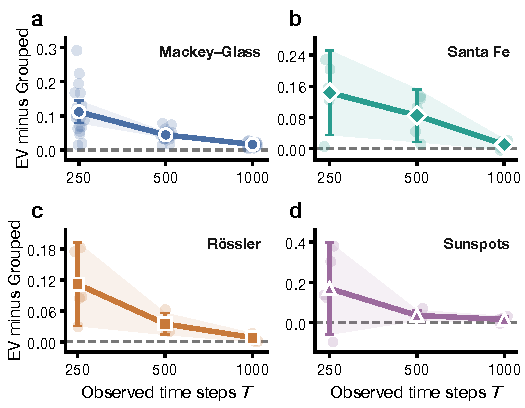
\includegraphics[width=\columnwidth]{fig3_regime_map.pdf}
  \caption{\fontsize{7.25}{8.0}\selectfont When aggregation helps most, at a fixed budget of ten thousand
  circuit executions. Each panel is one task. The vertical axis shows how much
  Grouped improves on full averaging, measured as the EV error minus the
  Grouped error, so a value above the dashed zero line means Grouped wins and a
  value on the line means a tie. Moving right spends the same budget on more
  time steps and therefore fewer shots at each step, from $40$ shots at $250$
  steps to $10$ shots at $1000$ steps. In every task the improvement is largest
  on the left and shrinks toward zero on the right. The message is simple.
  Grouping helps most when each step is measured many times and the series is
  short, because that is exactly when full averaging wastes the most training
  examples. Points are trajectory or window units, and markers with bars are
  means with $95\%$ intervals.}
  \label{fig:regimes}
\end{figure}

\subsection{Trading time steps against shots}

Figure~\ref{fig:regimes} compares three ways of spending the fixed budget. With
$40$ shots at each of $250$ time steps, Grouped improves every task by
$0.086$ to $0.170$. The interval stays above zero for Mackey--Glass, Santa Fe
laser, and R\"ossler, while the sunspot result varies across windows. When the
same budget is spread over $1000$ time steps with only $10$ shots each, the
gains shrink to between $0.008$ and $0.016$, and the interval stays above zero
only for Mackey--Glass and sunspots.

\subsection{Why the gain is regularization}

Cov-EV keeps EV features and adds a penalty based on how the shots fluctuate
together. At the balanced setting its mean error is $0.0021$ to $0.0116$ NRMSE
below Grouped, and only the R\"ossler interval excludes zero. This near-match
supports the regularization mechanism in Eq.~\eqref{eq:loss-decomposition}
rather than extra device information (Fig.~\ref{fig:controls}). Raw is less
accurate than EV on Mackey--Glass and R\"ossler and inconclusive on the two
real-world datasets. At fixed $k$, the exact two-term loss reproduces the
Grouped ridge fit to numerical precision; Cov-EV independently tunes the
strength of the full shot-covariance penalty.

Grouping is also robust to how the groups are drawn. Across twenty repeated
settings the average improvements are $-0.0064$ on Mackey--Glass, $0.1103$ on
Santa Fe laser, $0.0177$ on R\"ossler, and $0.0493$ on sunspots. Only the
sunspot interval stays above zero, reflecting the wide variation across
settings. Fixing one grouping across time instead of reshuffling at every step
changes the error by at most $0.0021$ NRMSE, with every interval containing
zero. The grouping convention therefore matters far less than ordinary
run-to-run variation. Figure~\ref{fig:controls} collects these controls.

\begin{figure}[t]
  \centering
  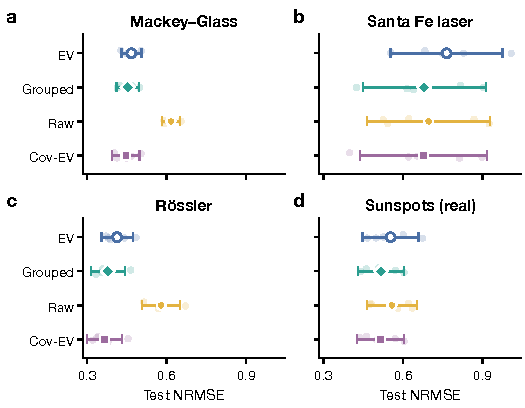
\includegraphics[width=\columnwidth]{fig4_controls_compact.pdf}
  \caption{\fontsize{7.25}{8.0}\selectfont Why the gain is regularization, shown task by task. Each panel places
  the four methods on the same error axis, where lower is better. Grouped (teal
  diamond) and Cov-EV (purple square) sit lowest and almost on top of each other
  on every task, EV (open circle) is behind them, and Raw (yellow, individual
  shots) is worst. The near-match between Grouped and Cov-EV is the key point.
  Cov-EV adds Grouped's fluctuation penalty directly to full averaging, so when
  it reaches the same error the benefit of grouping is regularization of the
  readout rather than extra information from the device. Faint points are the
  five trajectory or window means after repeated measurement trials are
  averaged within each unit. Markers and bars show the means and their $95\%$
  intervals. The order from top to bottom is EV, Grouped, Raw, and Cov-EV.}
  \label{fig:controls}
\end{figure}

\subsection{Transfer to hardware}

Figure~\ref{fig:hardware} reports the unmitigated hardware results. Grouped
improves every task, with mean gains from $0.038$ to $0.153$ NRMSE on
\emph{ibm\_fez} and from $0.031$ to $0.103$ on \emph{ibm\_marrakesh}. On Santa
Fe laser, the error falls from $0.750$ to $0.711$ on \emph{ibm\_fez} and from
$0.744$ to $0.713$ on \emph{ibm\_marrakesh}. Grouped is more accurate in $19$
of $20$ measurement blocks on each processor.

\begin{figure}[!b]
  \centering
  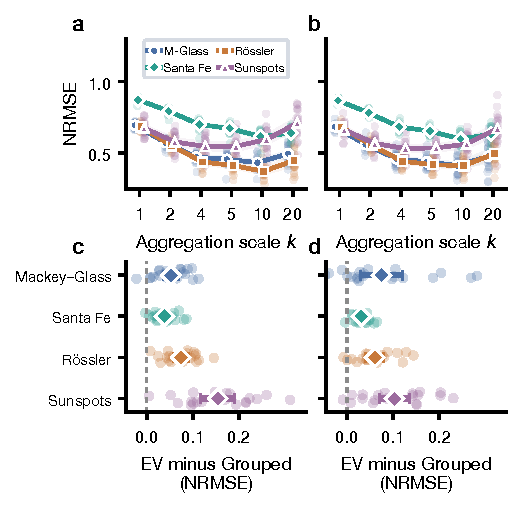
\includegraphics[width=\columnwidth]{fig5_hardware.pdf}
  \caption{\fontsize{7.25}{8.0}\selectfont The same effect on real hardware, on two processors. A separate
  ten-qubit reservoir was run without error mitigation on \emph{ibm\_fez} and
  \emph{ibm\_marrakesh}. For each task and processor, one acquisition of $400$
  shots at each of $T=500$ time steps was split into twenty disjoint records
  with $N=20$. (a,b)~The aggregation spectrum. On both devices the development
  error traces the same U shape over the aggregation scale $k$, so an
  intermediate scale again beats both endpoints on every task. (c,d)~The
  improvement per task, measured as the EV error minus the Grouped error, where
  the dashed line is a tie and points to its right favor Grouped. Grouped is
  more accurate on all four tasks on both machines. Faint points are the
  individual measurement blocks, and each colored marker with a bar is the mean
  with its $95\%$ interval. These intervals describe variation among the blocks
  of a single acquisition, not across independent hardware campaigns.}
  \label{fig:hardware}
\end{figure}

\section{Discussion}
\label{sec:discussion}

The main message is simple. A measurement record contains useful structure that
the standard expectation-value pipeline does not use for training, and a
validated choice of aggregation scale recovers part of it at no quantum cost.

Adaptive shot aggregation touches only the classical side of the pipeline. The
aggregation scale $k$ sets how many shots form each training view, and the two
familiar conventions remain available as its endpoints, Raw at one shot per view
and EV at all shots per view. The scale and ridge strength are chosen from
earlier time blocks, while the held-out test block remains unseen. No circuit is
rerun and no extra shots are spent.

The method helps most in a clear regime. When a record holds many shots at each
of relatively few time steps, full averaging turns a large measurement effort
into only a handful of training examples. Partial averaging spends those same
shots differently. It produces several lightly denoised views of each target,
and the small differences among the views act as a penalty that discourages the
readout from trusting feature directions dominated by measurement noise.
Equation~\eqref{eq:loss-decomposition} makes this exact. Grouped training is
ordinary averaging plus a penalty read from the observed shot fluctuations.

Our control confirms this reading. Cov-EV applies the same type of covariance
penalty after full averaging and reaches slightly lower mean error, yet stays
close to Grouped on every task. Their similar performance supports covariance
regularization as a shared mechanism. The small gap shows that grouping is one
convenient way to obtain this regularization, not the only one, and that the
benefit arises in the classical fit rather than from additional physical
information.

The effect also transfers. It appears in the six-qubit simulation reservoir and
again in a separate ten-qubit circuit on two processors, testing transfer across
reservoir designs rather than whether more qubits help.

A practical consequence follows. A different group size can only be built from
the individual shot outcomes, so trying other scales later is possible only if
those outcomes were kept. An experiment that stores just the averaged
expectation value has already thrown away the option to regroup, while an
experiment that keeps its full shot record leaves every group size open for
free.

The hardware results have a deliberately narrow scope. Their confidence
intervals are computed from the measurement blocks of one acquisition on each
task and processor. They therefore show that the effect is stable within a
single run, not that it repeats across separate runs on different days or
calibration settings. Confirming that reproducibility is the main open question,
and the natural next tests are independent hardware campaigns, other reservoir
families, and richer readouts.

\section{Conclusion}
\label{sec:conclusion}

Turning a shot record into training data has always involved a choice, and the
field has answered it by reflex, averaging everything. We show the reflex is
beatable. Choosing the aggregation scale by validation lowers mean test error
on chaotic and real-world forecasting at the balanced budget, holds on two
superconducting processors, and requires no additional quantum cost. Because
every measurement-based reservoir produces such a record, the choice we make
explicit here is available to any of them, and the question it raises belongs
to finite-shot learning in general.


\vspace*{-4pt}
\balance
\bibliographystyle{IEEEtranDoi}
\bibliography{bstcontrol,references}

\end{document}
